\chapter{Projecte de sensors}
\section{Experimentació}
Per comprendre millor com afecten els diferents paràmetres configurables corresponents a BLE i també les prestacions dels perifèrics de la placa es realitzaran els següents escenaris.

\subsection{ADC}
La placa té un convertidor analògic-digital que ens permetrà enviar senyals analògiques un cop s'han mostrejat.
Aquest ADC té x canals i una freqüència de mostreig de 200 Kmostres per segon.
Com que té x canals es poden 

En aquest treball no es tractaran directament els sensors sinó que es simularan le senyals que en sortirien.
Com que la placa i el seu ADC treballa a 3.3V es crearà un circuit que permeti controlar un voltatge d'entre 0 i 3.3V.

Aquest circuit es basarà en un divisor de voltatge simple format per una resistència i un potenciòmetre.
El potenciòmetre permet canviar la resistència del element a través d'un cargol i junt amb el circuit que l'envolta permetrà canviar el voltatge a la sortida.
\begin{figure}[!h]
	\begin{center}
		\begin{circuitikz}
			\draw
			(0,2) node[anchor=east] {$V_{in}$}
			to [R=$R_1$, *-] (2,2)
			to [vR=$R_{pot}$, *-] (2,0) node[tlground](GND){};
			\draw
			(2,2) to [short, -*] (3,2)
			to (3,2) node[anchor=west] (3,2) {$V_{out}$};
		\end{circuitikz}

	\end{center}
\end{figure}

Aquest circuit segueix la estructura d'un divisor de voltatge per tant es pot calcular el voltatge a la sortida segons la següent fórmula.

\begin{equation}
	V_{in}\cdot\frac{R_{pot}}{R_1+R_{pot}}=V_{out}
\end{equation}

Per escollir els components cal tenir in compte utilitzar resistències de valor alt per reduir el consum d'energia.
S'utilitzarà un potenciòmetre de 10KOhms per tant serà una resistència que es podrà modificar des de 0 Ohms fins 10 KOhms.
Per trobar la $R_1$ que compleixi els requisits queda la següent fórmula.

\begin{equation}
R_1=5V\cdot\frac{10k\Omega}{3.3V}-10k\Omega\approx5151\Omega
\end{equation}

Per a la $R_1$ s'utilitzaran resistències de la sèrie E12, els valors que més s'acosten a $5121\Omega$ són $5.6k\Omega$ i $4.6k\Omega$.
Per assegurar-se que no es superen els 3.3V a la entrada del ADC que podria fer malbé el dispositiu s'escull la resistència superior, per tant el circuit final quedarà de la següent manera.

\begin{figure}[!h]
	\begin{center}
		\begin{circuitikz}
			\draw
			(0,2) node[anchor=east] {$5\,V$}
			to [R=$5.6\;k\Omega$, *-] (2,2)
			to [vR=$ \lbrack 0-10 \rbrack \;k\Omega$, *-] (2,0) node[tlground](GND){};
			\draw
			(2,2) to [short, -*] (3,2)
			to (3,2) node[anchor=west] (3,2) {$[0-3.3]\;V$};
		\end{circuitikz}

	\end{center}
\end{figure}


\subsection{Abast}

Com s'ha mencionat anteriorment l'abast teòric que té BLE és considerable comparat amb les tecnologies similars.
Però cal entendre que al estar utilitzant la banda de 2.4 GHz, l'abast de BLE dependrà de l'entorn, on pot haver-hi molta variabilitat d'interferències.
És per això que en un escenari realista l'abast que es pot assolir pot ser molt diferent del teòric.
Les LAUNCHXL-CC1352R1 utilitzades per a aquest treball, per si soles, no són l'eina perfecte per fer proves d'abast.
Això es deu, en part, a que no es pot transmetre a la màxima potència permesa per l'estàndard que és de fins a 20 dBm.
Com a molt es pot transmetre a 5 dBm i per defecte es s'utilitzen 0 dBm de potència en transmissió.
Per realitzar un experiment que fos més precís seria avantatjós utilitzar una antena externa més directiva.
Enlloc d'analitzar l'abast de la tecnologia en aquest apartat es farà un balanç comparatiu per veure les diferències reals d'utilitzar les diferents capes físiques de BLE.

Per a aquest apartat es va realitzar un experiment pràctic en un lloc relativament aïllat i on es pogués tenir una suficient distància amb visibilitat directa.
Es va escollir un pàrquing i es va utilitzar la potència per defecte de 0 dBm per poder treballar amb distàncies més curtes.

\begin{figure}[!h]
	\begin{center}
		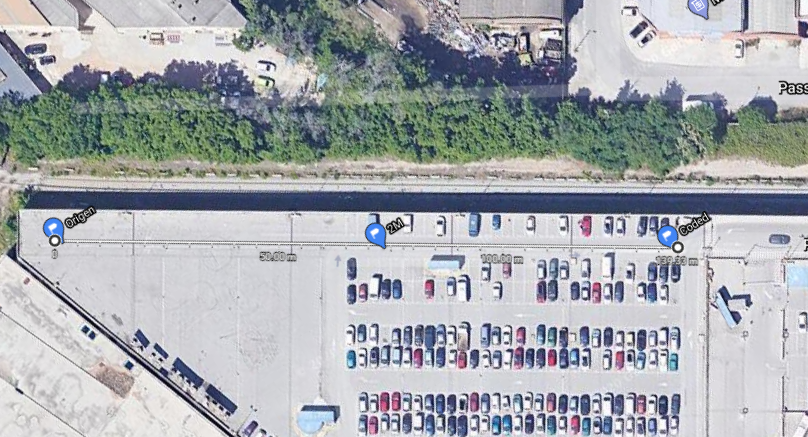
\includegraphics[width=\textwidth]{./images/prova_abast.png}
		\caption{Abast}
	\end{center}
\end{figure}

El procediment per realitzar l'experiment va ser deixar una de les plaques sobre un cotxe i amb l'altre connectada a una altre ordinador anar retrocedint fins que es perdés la connexió.
Per forçar que es perdés la connexió quan ja no es podia establir una comunicació des de la placa que s'anava movent s'anaven enviant peticions de lectura d'atributs.

El resultat va ser d'una distància màxima de 75 metres amb la capa física de 2M i de 135 metres quan s'utilitzava la capa Coded S=8.
S'analitzarant només aquestes capes físiques ja que al no haver-hi interferències significants i sempre es mantenia visibilitat directe els resultats de la capa 1M eren similars als de 2M i els de Coded S=2 eren similar als de S=8.

Amb aquest experiment s'ha validat tal i com s'havia comentat anteriorment els avantatges que aporta la nova capa física Coded que no existia abans de la versió 5.0 de BLE.

En aquest apartat només s'ha vist una de les millores de la capa física Coded però també cal recordar que on també és extremadament útil a part de l'abast és en el de resistència a les interferències.
Aquest component seria interessant poder-lo provar en un futur (queda per fer).


\subsection{Consum d'Energia}

El consum dels elements que utilitzen BLE és molt important ja que aquesta tecnologia està orientada a consumir la menor quantitat d'energia possible.
Les plaques que s'utilitzen per aquest projecte contenen una tecnologia anomenada EnergyTrace que permet veure quanta corrent s'està consumint en cada instant de temps.
D'aquesta manera es pot analitzar comparativament en quin moment s'està consumint l'energia i es poden adaptar els paràmetres de la connexió per veure quin serà l'estalvi que s'aconseguirà.
Així es poden prendre les decisions de quins sacrificis es poden suportar pel que fa a latència, per exemple, a canvi de reduir el consum.




\section{Mesures Biològiques}

Si es volen transmetre la velocitat dels batecs del cor això suposa, aproximadament, una mostra cada segon d'uns 10 bits més un instant de temps de 30 bits suposa uns 40 bits/segon, insignificant.

Si el que es vol es transmetre el senyal directament que prové del sensor que mesura la sang.
Considerem el màxim de 200 batecs per minut, això és una freqüència de 3,3 Hz, si mostregem a 10 vegades Fmax, 33 mostres/segon amb una resolució de 10 bits la tassa es de 330 bits/s

\section{ADC}


\section{Mesures mediambientals}
\subsection{Arquitectura}
